% Chapter 18: Ferromagnetic spins and the Ramanujan Vere-Jones laws as instruments. Sources: misc/reviews/nick-volume3/vol3/chE_ferro.tex 40-62, 165-203, 233-245, 265-277 and chF_ramanujan.tex 45-70, 311-516 (rule and toy table only), 651-670, 952-1142; report U11 (E1, E2, E3, E5, N1 to N5, R1 to R6 and minors), verification W5 V16; 17 Nov 2026.
\label{f:ch:ferro}\label{r:ch:ramanujan}

P\'olya wrote $\Xi$ as the characteristic function of a random variable. Lee and Yang, and later Newman, identified the ferromagnetic laws, whose moment generating functions have only imaginary zeros. RH asks that P\'olya's law be ferromagnetic. Ramanujan never wrote on RH, but one of his series, joined to the hyperbolic secant sums of Lai and Vere-Jones through the exit time of Brownian motion, gives a laboratory in which the finite tests of the earlier chapters can be compared. Material not found in Volumes I and II comes from an unrefereed note of Polson (November 2026).

\section{The dictionary, and two coupled spins}\label{f:sec:ly}

A law on the line is ferromagnetic if its moment generating function has only purely imaginary zeros. By Theorem~\ref{fm:thm:dual} an even law is ferromagnetic exactly when the reciprocal of its moment generating function, in the variable $u=w^2$, is the Laplace transform of a hitting time whose Thorin atoms are the squares of the zero ordinates. The standard laws are listed in Table~\ref{fm:tab:examples}, and the converse direction is Proposition~\ref{prop:rigid}.

The Lee and Yang theorem says that ferromagnetic couplings preserve the class. For spins $\sigma_i=\pm1$ with energy $-\sum J_{ij}\sigma_i\sigma_j$ and $J_{ij}\ge0$, the magnetisation $M=\sum\sigma_i$ is ferromagnetic. The smallest case can be pushed through the dictionary by hand.

\paragraph{A worked example: two coupled spins and their hitting time.} Two spins with coupling $J$ have $\E e^{zM}\propto e^{J}\cosh2z+e^{-J}$. Normalised, $\E\cosh(wM)=(e^{J}\cosh2w+e^{-J})/(e^{J}+e^{-J})$, whose zeros solve $\cosh2w=-e^{-2J}$. For $J\ge0$ define $\theta_J\in(\frac\pi2,\pi]$ by $\cos\theta_J=-e^{-2J}$. The zeros are $w=\pm\frac i2(\theta_J+2\pi k)$ and $w=\pm\frac i2(2\pi-\theta_J+2\pi k)$ for $k\ge0$. So the reciprocal of the moment generating function, in $u=w^2$, is the Laplace transform of a sum of independent exponential variables with rates, the Thorin atoms,
\[
\frac{(\theta_J+2\pi k)^2}{4}\quad\text{and}\quad\frac{(2\pi-\theta_J+2\pi k)^2}{4},\qquad k\ge0 .
\]
(Here the clock is half the exit time of standard Brownian motion, so that the exit of $(-1,1)$ has atoms $(2k+1)^2\pi^2/4$.) Two limits check the formula. When $J=0$ the spins are independent and $\theta_0=\pi$. Every atom $(2k+1)^2\pi^2/4$ appears twice, and the hitting time is the sum of two independent exits from $(-1,1)$, as $\E\cosh(wM)=\cosh^2w$ requires. As $J\to\infty$ the spins lock and $\theta_J\to\frac\pi2$. The two families interleave into the single family $(2m+1)^2\pi^2/16$, $m\ge0$, which is the exit from $(-2,2)$: the locked pair is one spin of size two. For $J<0$ there is no real $\theta_J$ and the atoms leave the axis. This is the Lee and Yang theorem in its smallest case, read on the side of the hitting time. The example is elementary and proved. We have not found it in the literature.

\section{The chain of the cosh spin}\label{f:sec:spinchain}

By Theorem~\ref{fm:thm:dual}, P\'olya's cosh spin $\Phi^*$ has a hitting time, and by Chapter~\ref{b:ch:chain} that hitting time has a birth and death chain whose spectral measure has atoms at $t_k^{-2}$, where $t_k$ are the zeros of $\Xi^*$. All its rates are positive, because the zeros are real. The question is how this chain compares with the chain of $\xi$. By Section~\ref{fm:sec:simple}, $\Phi^*$ keeps only the $e^{9u/2}$ part of the summand $n=1$ of the theta series, symmetrised, with $\exp(-\pi e^{2u})$ replaced by $\exp(-2\pi\cosh2u)$. It is not the summand $n=1$ of $\Phi$.

\begin{computation}\label{f:comp:spinchain}
A scan of $e^{\pi t/4}\,\Re K_{\frac94+\frac{it}2}(2\pi)$ with step $0.05$ finds $202$ zeros of $\Xi^*$ below height $400$, the same number as for $\Xi$ (double precision floating point).
\begin{enumerate}
\item Measured in mean spacings of the zeros of $\zeta$, the displacement of the $k$th zero of $\Xi^*$ from the $k$th smooth zero $\gamma_k^{\rm s}$ of Chapter~\ref{ch:progress} is $-0.74$ for $k=1$, $-0.11$ for $k=10$, $-0.04$ for $k=50$, $-0.02$ for $k=100$ and $-0.01$ for $k=202$.
\item From the $20$th zero on, the spacings of the zeros of $\Xi^*$, in units of the mean spacing, have relative standard deviation $0.002$ (computed), and for the zeros of $\Xi$ over the same range $0.366$.
\item With smooth zeros above height $400$, the chain of the cosh spin and the chain of the smooth zeros agree to within $0.001$ in $\log\alpha_j$ for every level $20\le j\le399$, and to $0.0003$ beyond level $100$ (computed). On levels $1$ to $20$ the difference has mean $0.14$ and standard deviation $0.35$, from the misplaced lowest zeros. The chain of $\Xi$ differs from the smooth chain by a fluctuation of standard deviation $0.080$, $0.065$, $0.046$ and $0.035$ on levels $1$ to $20$, $20$ to $100$, $100$ to $200$ and $200$ to $399$ (computed).
% UNVERIFIED: items 2 and 3 were not rerun in refereeing.
\end{enumerate}
\end{computation}

% UNVERIFIED: the lower panel of the figure (chain against smooth chain) was not rechecked; check the plotted normalisation of the rates against the chain chapter before printing.
\begin{figure}[ht]
\centering
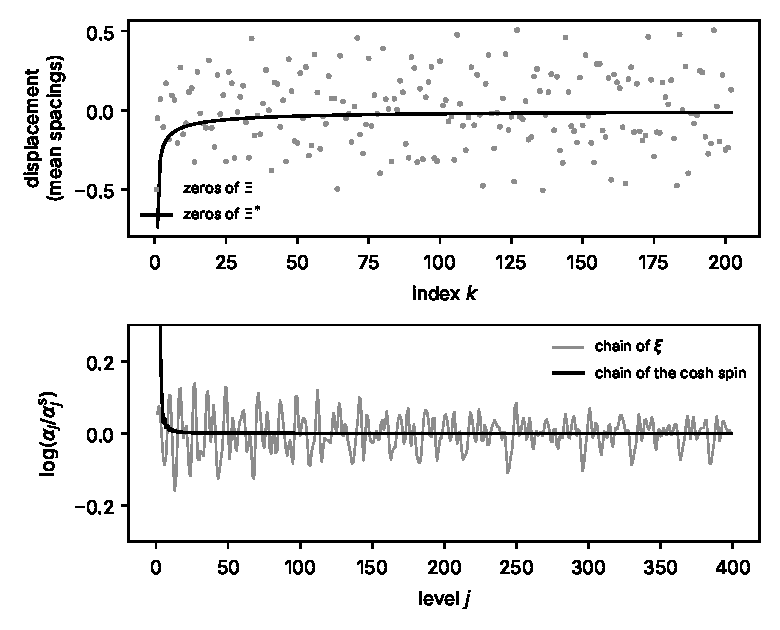
\includegraphics[width=\textwidth]{fig/v3/f_fig_spinchain.pdf}
\caption{Above: displacements of the zeros of $\Xi^*$ (line) and of $\Xi$ (points) from the smooth zeros of $\zeta$, in mean spacings. Below: the chain of the cosh spin and the chain of $\xi$, each against the chain of the smooth zeros.}\label{f:fig:spinchain}
\end{figure}

Figure~\ref{f:fig:spinchain} shows the two halves of the computation. P\'olya's approximant has its first zero far too low (Table~\ref{tab:biane:zeros}), but above the first few zeros its zeros follow the smooth zeros of $\zeta$, to a tenth of a spacing at the tenth zero and to a hundredth near the two hundredth, and its chain agrees with the Gamma chain of Chapter~\ref{b:ch:chain} to the accuracy stated. This is a computed agreement, not an identity.

This gives the fluctuation of route B a description. The chain of $\xi$ is the chain of a positive kernel $\Phi$, and the Gamma chain is, to the accuracy computed, the chain of the positive ferromagnetic kernel $\Phi^*$. The fluctuation $\varepsilon_j$ is therefore the effect on the chain of the difference $\Phi-\Phi^*$, which contains the rest of the summand $n=1$ (Proposition~\ref{fm:prop:psi}) and the sum over $n\ge2$, where the integers, and through them the primes, enter. In the language of Chapter~\ref{ch:progress}, the displacements $\delta\gamma_k$ that drive the linear response are, above the first few zeros and to the accuracy computed, the displacements of the zeros of $\Xi$ from those of $\Xi^*$. A proof of RH along this line would deform $\Phi^*$ into $\Phi$ so as to move real zeros without moving a pair off the line. The de Bruijn and Newman flow is one such deformation, and the Euler product would have to supply another.



\section{A protocol for testing a spin system}

Suppose someone proposes a family of spin systems, with ferromagnetic couplings built from the primes, whose magnetisation is meant to converge to P\'olya's law. The chapters of this volume suggest a protocol for deciding in an afternoon whether the proposal can be right. It is heuristic: it lists necessary checks, and no proof stands behind it.

\begin{enumerate}
\item Check the smooth part. The zeros of the moment generating function of the magnetisation should follow the smooth counting law, as those of the cosh spin do. If they do not, the proposal fails before the primes enter. The chain makes this quantitative: its rates should approach the Gamma chain at the levels where the zeros are dense.
\item Check the fluctuation. The zeros should be displaced from the smooth zeros by displacements of the size of those of the zeros of $\Xi$, of standard deviation $0.28$ mean spacings. By Computation~\ref{pp:comp:rigid} it is the single displacement distribution, not the long range rigidity, that the chain responds to, so this is the statistic to match first.
\item Check the control. The same construction applied to the coefficients of the Davenport and Heilbronn function, which has the same smooth part and no Euler product, must fail: either the couplings it produces are not all ferromagnetic, or the limit is not the control's kernel. A construction that gives ferromagnetic couplings for the control proves too much, since the control has zeros off the line.
\item Check sharpness along the heat flow. Replacing $\Phi$ by $e^{\lambda u^2}\Phi$ with small negative $\lambda$ must break the construction, by the theorem of Rodgers and Tao \cite{RodgersTao}.
\end{enumerate}

Step 1 is where P\'olya's approximant passes and step 2 is where it fails, by design. No proposal known to us passes all four.

\section{The heat flow as a family of spins}\label{f:sec:heat}

Newman \cite{Newman1976} introduced the constant that carries his name in the language of this chapter. Multiplying P\'olya's kernel by $e^{\lambda u^2}$ multiplies the law by a Gaussian factor: for $\lambda<0$ a Gaussian tilt toward the origin, for $\lambda>0$ a tilt away from it. De Bruijn proved that the property of being ferromagnetic is monotone along this family \cite{deBruijn}: if $e^{\lambda_0u^2}\Phi$ is ferromagnetic, so is $e^{\lambda u^2}\Phi$ for every $\lambda>\lambda_0$, and Newman proved that some tilt toward the origin is not ferromagnetic. So there is a finite threshold $\Lambda$, and RH is $\Lambda\le0$. Rodgers and Tao \cite{RodgersTao} proved Newman's conjecture $\Lambda\ge0$. In the language of spins: however weakly one tilts P\'olya's law toward the origin, by $e^{-\epsilon u^2}$, the result is not ferromagnetic. Equivalently, for every $\epsilon>0$ the reciprocal of the tilted moment generating function is not the Laplace transform of a generalised gamma convolution, because some of its would be Thorin atoms are not real and positive.

Three consequences for a ferromagnetic proof are worth stating.

\paragraph{No slack.} A construction that produced P\'olya's law as the magnetisation of a ferromagnetic system would have to break under every Gaussian tilt toward the origin. Systems whose ferromagnetism comes from inequalities with room to spare cannot do this unless the room disappears exactly at P\'olya's law (requirement 3 of Section~\ref{ch:pathdetail}).

% TODO (authors, M4): the Hurwitz wording in this paragraph and in the sharpness paragraph of the five requirements is ours; confirm.
\paragraph{A family of controls.} For each $\lambda<0$ the tilted law is a non ferromagnetic law built from $\Phi$ itself, with the same arithmetic. Conditional on RH, by Hurwitz's theorem the off line pairs of the tilted function leave every compact set as $\lambda\uparrow0$ unless they converge to a multiple real zero, so the rung of the ladder of Chapter~\ref{p:ch:path} at which the density fails would tend to infinity (heuristic; we have not proved it, and without RH off line zeros of the untilted function sit at fixed heights). By Chapter~\ref{ch:progress} the level of the chain at which a pair is seen grows like $3.3\,N(T)$ plus a term logarithmic in the distance of the pair from the line. So the family $e^{\lambda u^2}\Phi$, $\lambda<0$, would be a supply of controls of adjustable difficulty.

\paragraph{What the tilt does to the cosh spin.} The approximant $\Phi^*$ is ferromagnetic, and so is $e^{\lambda u^2}\Phi^*$ for $\lambda\ge\Lambda^*$, with its own constant. For the variable $P$ of Section~\ref{ch:biane}, Proposition~\ref{prop:biane:lambdaP} proves the constant finite and not positive, and notes that Newman's argument applies verbatim to $\Phi^*$. Computing $\Lambda^*$ is a finite problem that we have not carried out.

\section{Ramanujan and Vere-Jones: the sources}\label{r:sec:sources}

\paragraph{The 1915 paper on $\xi$ and $\Xi$.} In \emph{New expressions for Riemann's functions $\xi(s)$ and $\Xi(t)$} \cite{Ram15} Ramanujan gave integral representations of $\Xi$ against products of gamma functions. Open problem~\ref{r:op:Ram} returns to them.

\paragraph{The M\"obius formula reported by Hardy and Littlewood.} In their memoir of 1916 \cite{HL16}, Hardy and Littlewood attribute to Ramanujan a formula for the series $\sum_n\mu(n)n^{-1}e^{-x/n^2}$, with a transformation under $x\mapsto\pi^2/x$ that holds, under hypotheses on the zeros, with a sum over the zeros of $\zeta$, and observe that RH is equivalent to a rate of decay of the series. The formula is a Laplace mixture with signed weights, and the signs destroy the positivity the Thorin programme needs. Its hyperbolic secant form is Proposition~\ref{dl:prop:sechram}.


\paragraph{The lost notebook.} A transformation formula from the pages printed with the lost notebook gives a law whose characteristic function contains $\Xi$ (Theorem~\ref{dl:thm:Z} and Remark~\ref{dl:rem:Zid}).

\paragraph{Divisor series and Gauss sums.} In two short papers \cite{RamG,RamF} Ramanujan evaluated definite integrals connected with Gauss sums and proved closed forms for Dirichlet series such as $\zeta(s)^4/\zeta(2s)=\sum d(n)^2n^{-s}$.

\paragraph{Vere-Jones.} Lai and Vere-Jones studied the Meixner hypergeometric law, whose characteristic function is a power of a hyperbolic secant, and the sums of hyperbolic secants with M\"obius weights that arise when such laws are combined \cite{LVJ}. Those sums are the analogue of Ramanujan's Gaussian series, and Volume II joins the two (Proposition~\ref{dl:prop:sechram}, Theorem~\ref{rz:thm:sech} and Section~\ref{ri:sec:cauchy}).
\section{The exit time in three roles}\label{r:sec:vj}

Let $\tau$ be the exit time of standard Brownian motion from $(-1,1)$. It is the mixing variable of the worked example of Chapter~\ref{ch:cosine}, and the closing paragraph of Proposition~\ref{dl:prop:sechram} identifies its negative moments with the completed Dirichlet beta function. Write $\Lambda(s,\chi_4)=(\pi/4)^{-(s+1)/2}\Gamma(\frac{s+1}2)L(s,\chi_4)$, so that $\Lambda(s,\chi_4)=\Lambda(1-s,\chi_4)$.

\paragraph{Laplace transform: the eigenvalues.} $\E e^{-s\tau}=\sech\sqrt{2s}=\prod_{k\ge0}\bigl(1+s/\lambda_k\bigr)^{-1}$ with $\lambda_k=(2k+1)^2\pi^2/8$, the eigenvalues of $-\frac12\frac{d^2}{dx^2}$ on $(-1,1)$ with Dirichlet conditions. This is the Thorin form; the first row of Table~\ref{fm:tab:examples} lists $\tau/2$, with atoms $2\lambda_k$. The mean is $\E\tau=\sum_k1/\lambda_k=1$.

\paragraph{Wald identity: the hyperbolic secant law.} $\E e^{itH}=\sech t$ for $H=\sqrt\tau\,N$. Equivalently $\E\exp(tB_\tau-\frac12t^2\tau)=1$ with $B_\tau=\pm1$, the Wald couple of the spin and its exit time.

\paragraph{Mellin transform: an $L$ function.} $\E(\pi\tau/2)^{-s/2}=\Lambda(s,\chi_4)$. At $s=0$ and $s=1$ the right side is $1$: at $s=1$ because $\Lambda(1,\chi_4)=\frac4\pi\Gamma(1)\beta(1)=\frac4\pi\cdot\frac\pi4$. So $\E\tau^{-1/2}=\sqrt{\pi/2}$, a fact about Brownian motion that is Leibniz's series $1-\frac13+\frac15-\cdots=\frac\pi4$ in disguise.

\begin{proposition}\label{r:prop:sizebias}
Let $Y=(\pi\tau/2)^{-1/2}$. Then $\E Y=1$, and the size biased law of $Y$, with density $y$ times the density of $Y$, is the law of $1/Y$.
\end{proposition}

\begin{proof}
$\E Y=\Lambda(1,\chi_4)=1$. For the size biased variable $\tilde Y$, $\E\tilde Y^{\,s}=\E Y^{1+s}=\Lambda(1+s,\chi_4)$, while $\E Y^{-s}=\Lambda(-s,\chi_4)=\Lambda(1+s,\chi_4)$ by the functional equation. Both are Mellin transforms of positive laws that agree on a vertical strip, so the laws agree.
\end{proof}

The proposition is the probabilistic content of the functional equation of $L(s,\chi_4)$, as the theta identity is the content of the functional equation of $\zeta$ in the work of Biane, Pitman and Yor \cite{BPY01}. The zeta analogue, the size biased clock, is in Volume I. We have not found the statement for $\chi_4$ in the literature.

For $\tau$ the Thorin atoms are explicit and the zeros of its Mellin transform are not known to lie on a line. For the variable of Chapter~\ref{b:ch:chain} the situation is reversed: its Thorin atoms, if they exist, are the zeros, and RH asks that they exist. Open problem~\ref{r:op:V} asks whether one variable can do both jobs.

\paragraph{The Wald partner of the spin.} In the dictionary, $\tau/2$ is the hitting time attached to the ferromagnetic spin $\pm1$, the first row of Table~\ref{fm:tab:examples}. So the passage from Ramanujan's Gaussian series to the series of Lai and Vere-Jones is the passage from the Gaussian to its mixture over the Wald partner of the simplest ferromagnetic spin. It costs exactly one factor $\Lambda(s,\chi_4)$ in the Mellin transform and leaves the M\"obius signs untouched (Proposition~\ref{dl:prop:sechram}). A randomisation that removed the signs would need a variable whose negative moments vanish at the points $1-\rho$, a variable that already knows the zeros (the circle of Section~\ref{ch:pathdetail}).

% TODO (authors, M5): level of the chain (coefficient index j, e.g. c_148, level 74) and order of the Thorin ladder (near 75, ch:cand) are the same Hankel determinants in two indexings, so rows 2 and 3 of r:tab:measured and rows 3 and 4 of r:tab:depth report one measurement twice and the four instruments are three; the constant 3.3 N(T) appears in no Volume III chapter (1.7 = 75/43 is one point). Restructure the section, tables and the lines naming 3.3 and 1.7.
\section{Four instruments, four depths}\label{r:sec:connect}

The heat trace of the zeros, $k(x)=\sum_ze^{-z^2x}$ over the zeros $z$ with positive real part, gives a fourth finite ladder besides the three of the other chapters: the order $n$ of monotonicity, that is, positivity of $D_n(x)=\sum_zz^{2n}e^{-z^2x}$ for all $x>0$. Differentiating the explicit formula (Section~\ref{wt:sec:explicit}) $n$ times in $x$ turns each inequality $D_n>0$ into an inequality between a prime sum and an archimedean term, and RH is the full family. Every order up to $1.52\times10^{25}$ is proved by Theorem~\ref{ps:thm:free}, using the verified zeros below $3\times10^{12}$.

\begin{remark}[Which zeros does order $n$ see? Heuristic]\label{r:rem:rule}
The weight $t^{2n}e^{-t^2x}$ peaks at $t=\sqrt{n/x}$ with relative width $(4n)^{-1/2}$. A pair of zeros $u\pm iv$ off the line can make $D_n$ negative only when the weight isolates it from its real neighbours while its phase reaches $\frac\pi2$. This suggests the rule that $n$ is of order $\pi u^2/(4v\delta)$, where $\delta$ is the distance from $u$ to the nearest real ordinate. A toy model, the first $80$ zeros of $\zeta$ plus one artificial pair $u\pm iv$, gives the first failing order $613$ against $560$ from the rule at $u=27.7$, $v=0.4$, and $7752$ against $13355$ at $u=90$, $v=0.4$ (computed, not rerun in refereeing). So $n$ monotonicity probes zeros up to height about $\sqrt n$, and a pair at height just above $T$ (with $v$ near $\frac12$ and $\delta$ near the mean spacing) would first be seen at an order of size $T^2\log T$. The rule is not proved.
\end{remark}



For each instrument, Table~\ref{r:tab:depth} records the index that must be reached before a zero off the line at height $T$ can affect the test, where $N(T)$ is the number of zeros below $T$.

\begin{table}[ht]
\centering\small
\caption{How deep each finite test must go to see a zero at height $T$.}\label{r:tab:depth}
\begin{tabular}{@{}p{0.28\textwidth}p{0.3\textwidth}p{0.3\textwidth}@{}}
\toprule
instrument & index needed & source\\
\midrule
order of monotonicity of the heat trace & heuristic rule: of order $T^2\log T$ & Remark~\ref{r:rem:rule}\\[2pt]
rung of the ladder for $F$ & $N(T)+1$ & Theorem~\ref{p:thm:detect}\\[2pt]
level of the chain & about $3.3\,N(T)$, plus about $9\log_{10}(1/\eta)$ for a pair at distance $\eta$ & Remark~\ref{b:comp:dh} and Computation~\ref{pp:comp:coll}\\[2pt]
order of the Thorin ladder & about $1.7\,N(T)$ for the control & Chapter~\ref{c:ch:cand}\\
\bottomrule
\end{tabular}
\end{table}

The heat trace is the bluntest, since its index grows faster than the count of zeros. None of the four can be completed by computation. The sharp instruments buy resolution, not proof.

\subsection{The instruments measured on the control}

The indices in Table~\ref{r:tab:depth} are orders of magnitude. For the control and for the planted cosine model of Chapter~\ref{ch:cosine} they can be measured.

\begin{computation}\label{r:comp:heatdh}
% TODO (authors, M6): the zero set described (304 real zeros below 420 plus the pair 85.6993) cannot produce the second result (pair 114.1633, order 30124); the control has eight off line pairs below 400 (W5 V7). State the zero set of each run, rerun if needed; orders 8230 and 30124 are UNVERIFIED.
Take the heat trace over the zeros of the completed control function with positive real part: the $304$ on the line below height $420$ and the conjugate pair $85.6993\pm0.3085i$. Then $D_n(x)$ is positive for every $x$ for $n<8230$, and $D_{8230}(1.1525)<0$, with the weight peaking at height $84.5$. The rule of Remark~\ref{r:rem:rule}, with $u=85.70$, $v=0.3085$ and $\delta=1.948$ to the nearest real ordinate, predicts $9597$. For the second pair, $114.1633\pm0.1508i$ with $\delta=1.787$, the rule predicts $37979$, and the first failure found, in a search over orders $20000$ to $45000$, is at order $30124$, with the weight peaking at height $115.4$. The rule overestimates by $17$ and $26$ per cent (control values computed).

For the planted cosine model, real zeros at the odd multiples of $\frac\pi2$ (400 terms) and a pair $3\pm di$, the first failing order is $10$, $19$, $35$ and $67$ for $d=0.4$, $0.2$, $0.1$ and $0.05$, against $12$, $25$, $49$ and $99$ from the rule (floating point scan over $0<x<3n$; not a certificate). The rule overestimates by $20$ to $48$ per cent, and the product $nd$ falls from $4.0$ to $3.35$, so the growth is slightly slower than $1/d$.
\end{computation}
% UNVERIFIED: the control orders 8230 and 30124 were not rerun in refereeing.

% UNVERIFIED: the figure plots the control (n = 8000, 8230, 8500); the control numbers were not rerun.
\begin{figure}[ht]
\centering
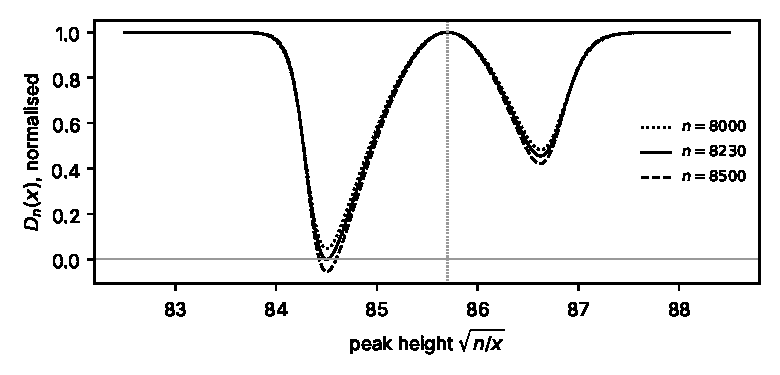
\includegraphics[width=\textwidth]{fig/v3/r_fig_heatdh.pdf}
\caption{$D_n(x)$ for the control, divided by the sum of the absolute values of its terms, against the height $\sqrt{n/x}$ at which the weight peaks, for $n=8000$, $8230$, $8500$. At $n=8230$ the dip just below the pair at $85.70$ first crosses zero.}\label{r:fig:heatdh}
\end{figure}

% r_fig_depth.pdf is NOT included: its left panel plots the draft's first failing orders (12, 22, 43, 84) with the line 4.8/d, which verification V16 found wrong (10, 19, 35, 67). It must be redrawn from the corrected orders; the right panel (chain of zeta, first negative rate against eta at height 415) was not rechecked.

As $n$ grows the weight narrows, the contribution of the real zeros near the pair falls, and the oscillating term of the pair, whose phase turns with $x$, pulls $D_n$ below zero at a point slightly below the pair, where the neighbouring real zeros are furthest away (Figure~\ref{r:fig:heatdh}). Table~\ref{r:tab:measured} puts these numbers beside the other instruments.

% UNVERIFIED: rung 44, Thorin ladder near 75, chain level 148 (control) and 2, 5 (planted cosine) are the draft's, not rerun (V17 rung 43 and 44 minors not done). The convention for the level index (coefficient j against level n = j/2, N10) must be matched with the chain chapter.
\begin{table}[ht]
\centering\small
\caption{The index at which each instrument first sees a pair off the line.}\label{r:tab:measured}
\begin{tabular}{@{}p{0.32\textwidth}p{0.24\textwidth}p{0.3\textwidth}@{}}
\toprule
instrument & control, pair at $85.70$ & planted cosine, pair $3\pm0.4i$\\
\midrule
rung of the ladder for $F$ & $44$ & $2$\\[2pt]
order of the Thorin ladder & near $75$ & not computed\\[2pt]
level of the chain & $148$ & $5$\\[2pt]
order of the heat trace & $8230$ & $10$\\
\bottomrule
\end{tabular}
\end{table}

\begin{table}[ht]
\centering\small
\caption{How the index grows as the pair approaches the line.}\label{r:tab:distance}
\begin{tabular}{@{}p{0.32\textwidth}p{0.55\textwidth}@{}}
\toprule
instrument & growth as the distance $d$ to the line shrinks\\
\midrule
rung of the ladder for $F$ & none: always $m+1$, but at shifts of order $\pi/d$ and in minors of size $e^{-c/d}$ (Corollary~\ref{p:cor:scale})\\[2pt]
level of the chain & logarithmic: about nine levels for each factor of ten in $d$ (Computation~\ref{pp:comp:coll})\\[2pt]
order of the heat trace & slightly slower than $1/d$: $10$, $19$, $35$, $67$ for $d=0.4$ to $0.05$ (Computation~\ref{r:comp:heatdh})\\
\bottomrule
\end{tabular}
\end{table}

The ordering is the same in both examples, and the tables say three different things about how a violation of RH would be found. The density sees a violation at the smallest index, but only after a shift that grows like $1/d$, in quantities that are exponentially small. The chain sees it at an index proportional to the number of zeros below it, with a correction only logarithmic in $1/d$, and in quantities of ordinary size, at the price of high precision. The heat trace sees it last, at an index growing roughly like the square of the height and nearly like $1/d$.

\section{Is there a path to RH?}\label{r:sec:path}

For the material of this chapter, no. Every statement that touches RH is one of four kinds.

\begin{enumerate}
\item A restatement. Proposition~\ref{prop:rigid} is RH in other words at the centre of the strip, and the law of Theorem~\ref{dl:thm:Z} has its singularities on the opposite half line from the zeros.
\item A positivity confined to absolute convergence. Proposition~\ref{dl:prop:deligne} gives positive L\'evy measures for $\sigma>1$. They sit on the lattice $\{m\log p\}$ and are not of Thorin form, and the zeros lie to the left of the pole at $s=1$, where the positivity gives only a bound by the value on the real axis.
\item A positivity that is too weak. RH is complete monotonicity of the Thorin function of the reciprocal Xi law, the same property at every order. Order $n$ sees zeros to height about $\sqrt n$ (Remark~\ref{r:rem:rule}, heuristic), so each finite order, such as the orders to $1.52\times10^{25}$ of Theorem~\ref{ps:thm:free}, is settled by a finite verification of zeros, and the passage to all orders is RH itself. This locates RH exactly. It does not approach it.
\item A signed identity. Proposition~\ref{dl:prop:sechram} is exact, and it shows that passing from Gaussian to hyperbolic secant kernels is a GGC randomisation costing one factor $\Lambda(s,\chi_4)$. The M\"obius signs are untouched.
\end{enumerate}



\subsection{The five requirements}

Section~\ref{ch:pathdetail} gave five requirements that any proof along the paths of this volume must meet. The results of this chapter can be checked against them.

\paragraph{The Euler product.} Proposition~\ref{dl:prop:deligne} is the only result here that uses it for positivity. It gives positive L\'evy measures for $\sigma>1$, where the Euler product converges, and says nothing at or below $\sigma=1$.
\paragraph{Uniformity in the height.} The finite orders of monotonicity are uniform in $x$ but not in the order $n$: each order is settled by a verification of the zeros below a height of order $\sqrt n$, and the proof of Theorem~\ref{ps:thm:free} uses exactly such a verification.

\paragraph{Sharpness along the heat flow.} The heat trace of $H_t$ for $t<0$ fails to be completely monotone if $H_t$ has zeros off the line, and by Computation~\ref{r:comp:heatdh} and the rule of Remark~\ref{r:rem:rule} the failure would appear at an order of the size of the square of the height of the colliding pair divided by its distance from the line (heuristic). Whether every finite order holds for $H_t$ when $|t|$ is small enough is not known.


\paragraph{Kernel positivity.} The variable of Theorem~\ref{dl:thm:Z} has a positive density for an unconditional reason, the positivity of $|\Xi|^2$, and this positivity does not distinguish $\zeta$ from the control, whose completed function is also real on the line.

\paragraph{Approximation.} The exit time randomisation of Proposition~\ref{dl:prop:sechram} is exact rather than approximate, so the fifth requirement does not arise.


\section{Open problems}

\begin{openproblem}\label{f:op:ferro}
Find a sequence of ferromagnetic spin systems whose magnetisations converge to P\'olya's law, starting from the cosh spin and adding one Euler factor at a time. Test each stage on the zeros of $\Xi^*$ in Table~\ref{tab:biane:zeros}.
\end{openproblem}

\begin{openproblem}\label{r:op:deform}
Computation~\ref{f:comp:spinchain} shows that the chain of P\'olya's cosh spin agrees with the Gamma chain beyond the first few levels. The kernel $\Phi^*$ is not the first term of $\Phi$ (Section~\ref{fm:sec:simple}), so $\Phi$ is not $\Phi^*$ plus the terms $n\ge2$. Deform instead: put $\Phi_\lambda=(1-\lambda)\Phi^*+\lambda\Phi$ for $\lambda\in[0,1]$, a positive even density at each $\lambda$, and follow the zeros of its transform and the rates of its chain as $\lambda$ increases from $0$, where all zeros are real, to $1$, which is the case of $\xi$. RH is the statement that all zeros are real at $\lambda=1$. By Lemma~\ref{pp:thm:pair} and Computation~\ref{pp:comp:coll}, the first pair to leave would be seen as two negative rates at a level set by its height (computed).
\end{openproblem}

\begin{openproblem}
Prove the converse of the heat trace rule with constants: if $D_n(x)>0$ for all $x$ and all $n\le n_0$, then all zeros with ordinate below $c\sqrt{n_0}$ are on the line. With the explicit formula (Section~\ref{wt:sec:explicit}) this would turn each $D_n>0$ into a verification of RH to a finite height by an inequality on primes.
\end{openproblem}

\begin{openproblem}\label{r:op:Ram}
Other identities in Ramanujan's 1915 paper \cite{Ram15} give integrals of $\Xi(\frac{t+is}{2})\Xi(\frac{t-is}{2})$ against gamma weights. For which weights is the density an EGGC characteristic function, so that the argument of Theorem~\ref{dl:thm:Z} yields further laws?
\end{openproblem}

\begin{openproblem}\label{r:op:V}
Replace the exit time $\tau$ in the randomisation of Proposition~\ref{dl:prop:sechram} by a general GGC $V$ and put $Q_V(x)=\E R(\frac12x^2V)$, where $R(y)=\sum_n\mu(n)n^{-1}e^{-y/n^2}$ is Ramanujan's series, with Mellin transform $\frac12\Gamma(\frac s2)\E(V/2)^{-s/2}/\zeta(1-s)$. Is there a $V$ whose negative moments cancel zeros of $\zeta(1-s)$ in part of the strip? This requires $\E V^{-s/2}$ to vanish at points $1-\rho$, so $V$ must itself encode zeros. The natural candidates are the Biane, Pitman and Yor variables.
\end{openproblem}

\begin{openproblem}
Explain the constant in the rule of Remark~\ref{r:rem:rule}. On the control it overestimates the first failing order by $17$ and $26$ per cent, and on the planted cosine model by $20$ to $48$ per cent, increasing as $d$ falls. A derivation from the phase of the term of the pair and the Gaussian approximation of the weight should give the constant and the correct dependence on $d$.
\end{openproblem}

\begin{openproblem}
Extend the first line of Proposition~\ref{dl:prop:deligne} to the completed function $(2\pi)^{-s}\Gamma(s)L(s,\Delta)$ and test numerically whether its reciprocal in the variable $6+\sqrt s$ has a nonnegative Thorin type representation, using the verified zeros of Keiper \cite{Keiper96}.
\end{openproblem}
